
\subsection{Inkrementell}
Aufgaben werden in fachlich abgeschlossene Teile eingeteilt.\\
Jedes Teilsystem (\textit{Inkrement}) wird so gewählt, dass es lauffähig und funktionstüchtig ist: Die Entwicklung der einzelnen Inkremente wiederum findet bspw. nach dem Wasserfallmodell statt,
wobei die Überführung in die letzte Phase ``\textit{Betrieb}`` dann wieder eine einzelne Phase ist, in der alle Teilsysteme zusammengeführt werden.\\
Die Auslieferung der einzelnen Inkremente an den Kunden findet bereits nach Fertigstellung derselben statt (vgl. Abbildung~\ref{fig:inkrementell}).\\

\begin{figure}
    \centering
    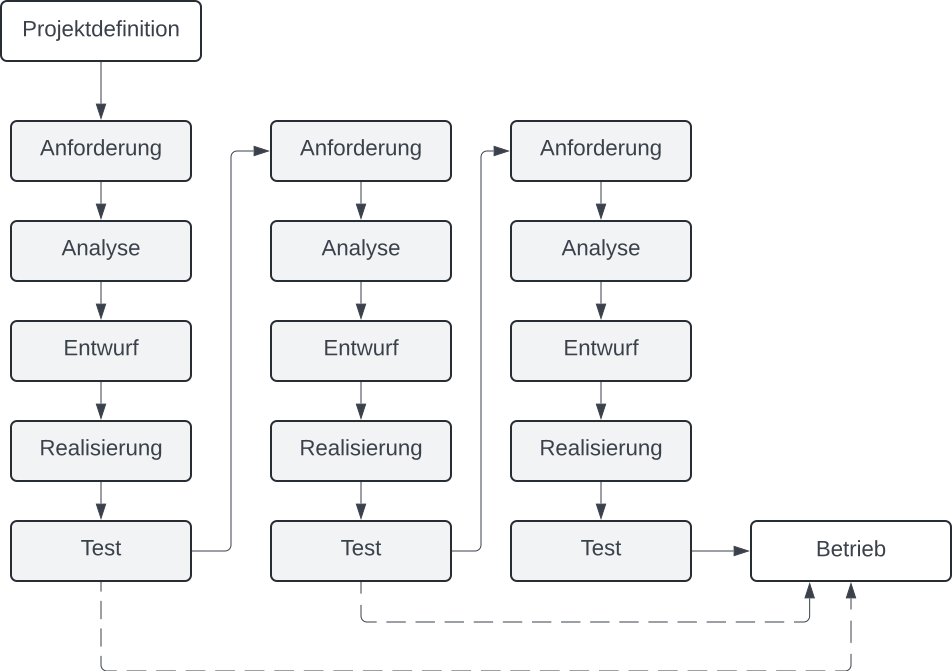
\includegraphics[scale=0.4]{part one/Prozessmodelle/img/inkrementell}
    \caption{Inkrementelles Phasenmodell.
    Nach der Integration und den Tests gehen die einzelnen Inkremente über in den Betrieb.
        (Quelle: in Anlehnung an \cite[322]{AABG14n})}
    \label{fig:inkrementell}
\end{figure}

\noindent
In Deutschland ist die bekannteste inkrementelle Vorgehensweise das \textbf{V-Modell XT}\footnote{ \textit{XT = eXtreme Tailoring}.
Eine ausführliche Beschreibung des Models liefert \textit{Balzert} in \cite{Bal08}. S. a.
\url{https://www.cio.bund.de/Webs/CIO/DE/digitaler-wandel/Achitekturen_und_Standards/V_modell_xt/v_modell_xt-node.html}, abgerufen 04.04.2024
}.\\
Das inkrementelle Vorgehen wird oft mit anderen Konzepten kombiniert.

\subsubsection*{Vorteile}

\begin{itemize}
    \item Kunde kann einzelne Teilsysteme abnehmen, ohne auf die Auslieferung des Gesamtsystems warten zu müssen.
    \item Durch Anwendung der Teilsysteme durch den Kunden kann dieser die Entwicklung der nächsten Inkremente beeinflussen.
    \item Entwickler können ihr Wissen aus den vorangegangenen Inkremente in die nächsten einfliessen lassen.
\end{itemize}

\subsubsection*{Nachteile}

\begin{itemize}
    \item Dauer der Entwicklung mit Inkrementen ist recht lange, da ein einzelnes Inkrement ein lieferfähiges Produkt darstellt, dass dieselben Phasen durchläuft wie ein einzelnes System, das über das Phasenmodell entwickelt wird
    \item Anforderungen des Kunden fließen nach der Anforderungsphase erst wieder in das nächste Inkrement ein
    \item Auch Entwickler, die während der Realisierung Schwächen im Entwurf entdecken, können Korrekturen erst im nächsten Inkrement einbringen.
\end{itemize}

\subsubsection*{Abgrenzung zum evolutionären Modell}
Obwohl Rückmeldungen des AG in die Entwicklung nachfolgender Inkremente einfliessen, wird zu Beginn des Projekts in der Anforderungsphase eine vollständige Anforderungsdefinition durchgeführt.\\
Erst dadurch ist es möglich, das Projekt in Inkremente zu unterteilen (vgl.~\cite[529]{Bal08}).\\

\noindent
Das \textbf{evolutionäre Modell} hingegen sammelt die Anforderungen im Laufe der Entwicklung: ``I can't tell you what I want, but I'll know it when I see it.`` (vgl. \cite[530]{Bal08}).